% ============================================================
%  chapter02.tex — 第二章 平面奇点
%  对应原书第二章。
%  研究平面自治系统平衡点的分类与判定：线性近似、非线性扰动、
%  中心—焦点判别、几何分类及零特征根情形。
% ============================================================

\setchapterimage{}
\setchapterintro{}
\chapter{平面奇点}

\newcommand{\chTwoFigurePlaceholder}[1]{%
  \begin{center}
    \fbox{\parbox{0.72\textwidth}{\centering\vspace{2.7cm}图~#1\\（图片占位）\vspace{2.7cm}}}
  \end{center}%
}

% ============================================================
%  §1  奇点和常点
% ============================================================
\section{奇点和常点}

给定微分方程组
\[
\left\{
\begin{aligned}
\dfrac{dx}{dt}&=X(x,y),\\
\dfrac{dy}{dt}&=Y(x,y),
\end{aligned}
\right.\tag{1.1}
\]
其中 $X(x,y),Y(x,y)\in C^0(D)$，$D\subseteq\mathbb{R}^2$。方程组(1.1)在奇点及常点有完全不同的性质。

从解析的观点看，若 $P_0(x_0,y_0)\in D$ 满足
\[
X^2(x_0,y_0)+Y^2(x_0,y_0)=0,
\]
则称 $P_0$ 为方程组(1.1)的一个奇点。这时 $x=x_0,y=y_0$ 是方程组(1.1)的一个解。若
\[
X^2(x_0,y_0)+Y^2(x_0,y_0)\ne0,
\]
则称 $P_0$ 为方程组(1.1)的一个常点。从拓扑的观点看，奇点是方程组(1.1)所定义的向量场在 $P_0$ 点的向量 $(X,Y)$ 为零的点；常点则是该向量不为零的点。从力学的观点看，若 $x$ 表示位置，则 $dx/dt$ 表示速度，$dy/dt=d^2x/dt^2$ 表示加速度；奇点是平衡位置，常点不是平衡位置。

\subsection*{常点附近轨线的拓扑结构}

在常点 $P_0$ 的邻域内，经一个非退化的线性坐标变换，可把 $P_0$ 移至原点，并使向量场在原点的方向为 $y$ 轴的方向。为简单起见，设方程组(1.1)满足
\[
x_0=y_0=0,\qquad X(0,0)=0,\qquad Y(0,0)\ne0.
\]
在充分小的圆邻域 $S(O,\varepsilon)$ 内 $Y(x,y)\ne0$，方程组(1.1)等价于
\[
\dfrac{dx}{dy}=\dfrac{X(x,y)}{Y(x,y)}.\tag{1.2}
\]
它的解可写成 $x=x(y,a)$，其中 $x(0,a)=a$。

\begin{center}
\begin{tikzpicture}[x=0.92cm,y=0.92cm,>=Stealth,font=\small]
  % 左图：参数直线族所在的长方形
  \draw[->] (-3.75,0) -- (-0.35,0) node[right] {$x$};
  \draw[->] (-2.05,-2.05) -- (-2.05,2.05) node[above] {$y$};
  \node[below left] at (-2.05,0) {$O$};
  \draw[thick] (-3.15,1.25) rectangle (-0.95,-1.25);
  \node[above left] at (-3.15,1.25) {$A$};
  \node[above right] at (-0.95,1.25) {$B$};
  \node[below right] at (-0.95,-1.25) {$C$};
  \node[below left] at (-3.15,-1.25) {$D$};
  \foreach \xx in {-2.75,-2.38,-1.62,-1.25}
    \draw[thick] (\xx,-0.82) -- (\xx,0.82);
  \draw[thick] (-1.62,-0.82) -- (-1.62,0.82);
  \draw[densely dashed,->] (-0.05,0.63) -- (-1.62,0.17);
  \node[anchor=west] at (-0.02,0.68) {$(a,0)$};
  \draw[densely dashed,->] (-0.08,-0.48) -- (-1.62,-0.48);
  \node[anchor=west] at (-0.02,-0.48) {$x=a$};

  % 右图：微分同胚下的曲边四边形及积分曲线族
  \draw[->] (0.55,0) -- (5.75,0) node[right] {$x$};
  \draw[->] (3.15,-2.05) -- (3.15,2.05) node[above] {$y$};
  \node[below left] at (3.15,0) {$O$};
  \draw[thick] (1.82,1.23) .. controls (2.55,1.18) and (4.26,1.17) .. (4.95,1.20);
  \draw[thick] (1.20,-1.26) .. controls (2.20,-1.20) and (3.75,-1.19) .. (4.47,-1.23);
  \draw[thick] (1.20,-1.26) .. controls (1.52,-0.50) and (1.37,0.55) .. (1.82,1.23);
  \draw[thick] (4.47,-1.23) .. controls (4.79,-0.42) and (4.63,0.50) .. (4.95,1.20);
  \draw[thick] (1.47,-1.24) .. controls (2.03,-0.56) and (1.72,0.50) .. (2.34,1.20);
  \draw[thick] (2.12,-1.22) .. controls (2.62,-0.42) and (2.38,0.46) .. (2.85,1.19);
  \draw[thick] (2.78,-1.21) .. controls (3.48,-0.44) and (3.05,0.42) .. (3.52,1.18);
  \draw[thick] (3.45,-1.21) .. controls (3.92,-0.34) and (3.73,0.45) .. (4.18,1.18);
  \draw[thick] (4.02,-1.22) .. controls (4.52,-0.36) and (4.22,0.48) .. (4.67,1.19);
  \node[above left] at (1.82,1.23) {$A'$};
  \node[above right] at (4.95,1.20) {$B'$};
  \node[below right] at (4.47,-1.23) {$C'$};
  \node[below left] at (1.20,-1.26) {$D'$};
  \draw[densely dashed,->] (5.22,0.66) -- (3.69,0.14);
  \node[anchor=west] at (5.24,0.72) {$(a,0)$};
  \draw[densely dashed,->] (5.18,-0.48) -- (3.73,-0.48);
  \node[anchor=west] at (5.22,-0.48) {$x=x(y,a)$};
\end{tikzpicture}
\captionof{figure}{常点邻域内平行直线族与积分曲线族的对应}
\end{center}


变换
\[
T:(a,y)\longmapsto (x(y,a),y)
\]
把矩形 $ABCD$ 一一地变为曲边四边形 $A'B'C'D'$，并把平行直线族 $x=a$ 变为积分曲线族 $x=x(y,a)$。若 $X,Y\in C^r(D)$，$r\ge1$，由第一章\S1可知 $T\in C^r(y,a)$。现证明 $T^{-1}\in C^r$。

由(1.2)，
\[
\dfrac{d(\partial x/\partial a)}{dy}
=\dfrac{Y\dfrac{\partial X}{\partial x}-X\dfrac{\partial Y}{\partial x}}{Y^2}
\dfrac{\partial x}{\partial a}.
\]
故
\[
\dfrac{d}{dy}\left\{\dfrac{\partial x}{\partial a}
\exp\left[-\int_0^y
\dfrac{YX_x-XY_x}{Y^2}\,dy\right]\right\}=0.
\]
又因 $x(0,a)=a$，所以
\[
\dfrac{\partial x}{\partial a}
=\exp\left\{\int_0^y\dfrac{YX_x-XY_x}{Y^2}\,dy\right\}\ne0.
\]
因此存在反变换
\[
T^{-1}:(x,y)\longmapsto (a(x,y),y),\qquad a(x,0)=x,
\]
它把积分曲线变为直线 $x=a$；由反函数定理 $T^{-1}\in C^r(x,y)$。所以，当 $X,Y\in C^r(D)$，$r\ge1$ 时，常点 $P_0$ 的充分小邻域内的积分曲线可经一个 $C^r$ 微分同胚变为一族平行直线。常点附近的拓扑结构是简单的；奇点附近的情形则复杂得多。

% ============================================================
%  §2  常系数线性方程组的奇点
% ============================================================
\section{常系数线性方程组的奇点}

考虑常系数线性方程组
\[
\left\{
\begin{aligned}
\dfrac{dx}{dt}&=ax+by,\\
\dfrac{dy}{dt}&=cx+dy.
\end{aligned}
\right.\tag{2.1}
\]
其中 $a,b,c,d$ 均为实数。其特征方程为
\[
D(\lambda)=\begin{vmatrix}a-\lambda&b\\c&d-\lambda\end{vmatrix}
=\lambda^2-(a+d)\lambda+ad-bc=0.
\]
令 $p=-(a+d)$，$q=ad-bc$，则 $D(\lambda)=\lambda^2+p\lambda+q$，
\[
\lambda_{1,2}=\dfrac{-p\pm\sqrt{p^2-4q}}{2}.
\]
以下讨论原点的九种情形。

\textbf{1.}\ $q<0$。特征根为异号实根。若 $c\ne0$，取
\[
x'=-cx+(a-\lambda_1)y,\qquad y'=-cx+(a-\lambda_2)y;\tag{2.2}
\]
若 $b\ne0$，取
\[
x'=(d-\lambda_1)x-by,\qquad y'=(d-\lambda_2)x-by.\tag{2.3}
\]
方程组化为
\[
\dfrac{dx'}{dt}=\lambda_1x',\qquad
\dfrac{dy'}{dt}=\lambda_2y'.\tag{2.4}
\]
解为 $x'=C_1e^{\lambda_1t}$，$y'=C_2e^{\lambda_2t}$，从而
\[
y'=C_3|x'|^{\lambda_2/\lambda_1},\qquad \lambda_2/\lambda_1<0.
\]
除两坐标轴外，轨线在两个方向均趋于无穷远；原点为鞍点。

\begin{center}
	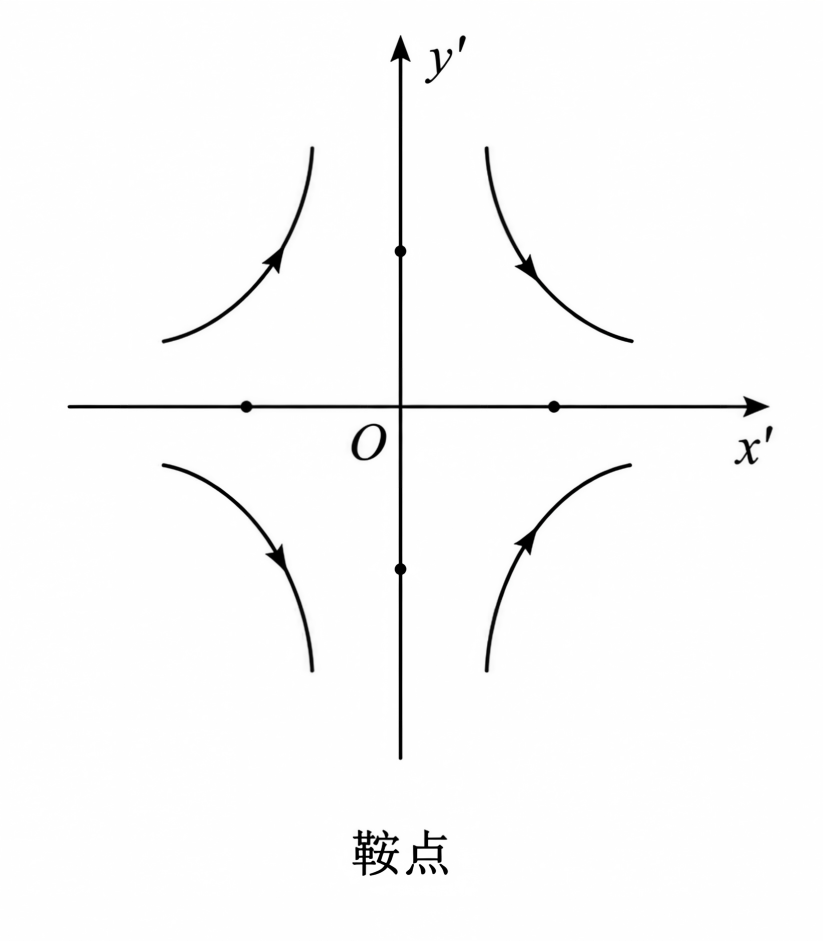
\includegraphics[width=0.4\linewidth]{figure/2.2}
	\captionof{figure}{鞍点}
\end{center}


\textbf{2.}\ $q>0,p>0,p^2-4q>0$。两个特征根均为负实根。由(2.2)或(2.3)化为(2.4)，此时 $\lambda_2/\lambda_1>0$，当 $t\to+\infty$ 时所有轨线均趋于原点。原点为稳定结点。

\begin{center}
	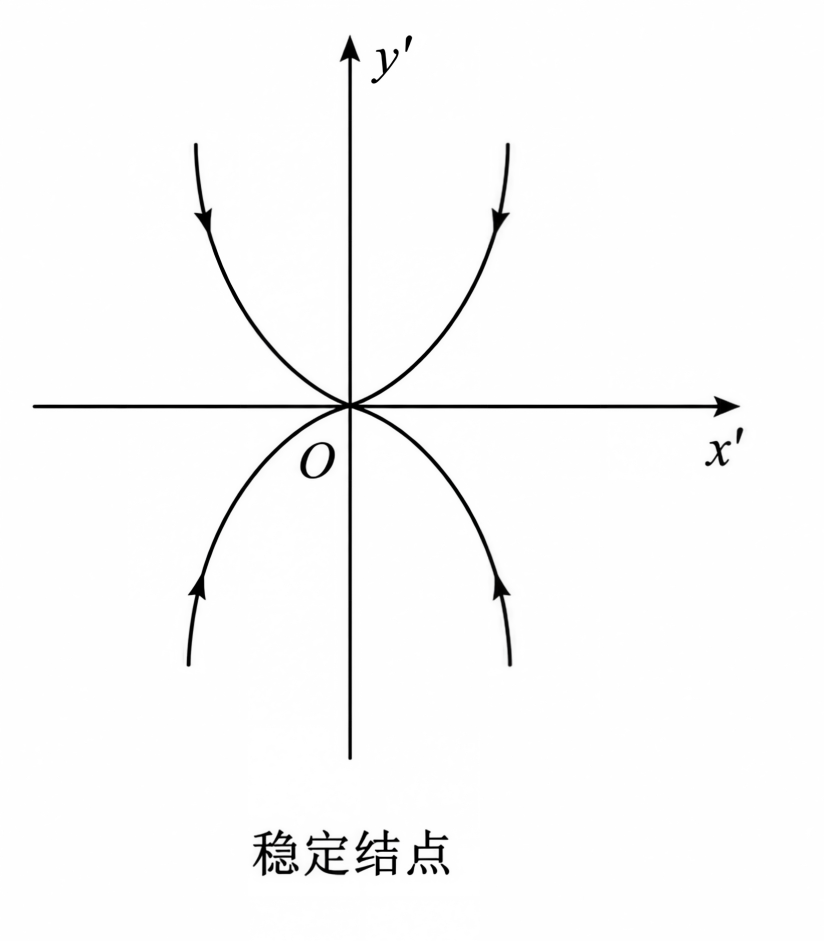
\includegraphics[width=0.4\linewidth]{figure/2.3}
	\captionof{figure}{稳定结点}
\end{center}


\textbf{3.}\ $q>0,p>0,p^2-4q<0$。特征根为
\[
\mu_1\pm i\mu_2,\qquad \mu_1=-\dfrac p2<0,
\]
并可化为
\[
\dfrac{dx'}{dt}=\mu_1x'+\mu_2y',\qquad
\dfrac{dy'}{dt}=-\mu_2x'+\mu_1y'.\tag{2.5}
\]
令 $x'=r\cos\theta,y'=r\sin\theta$，得
\[
\dfrac{dr}{dt}=\mu_1r,\qquad \dfrac{d\theta}{dt}=-\mu_2.\tag{2.6}
\]
故 $r=r(0)e^{\mu_1t}$，$\theta=-\mu_2t+\theta(0)$，所有轨线螺旋形趋于原点；原点为稳定焦点。

\begin{center}
	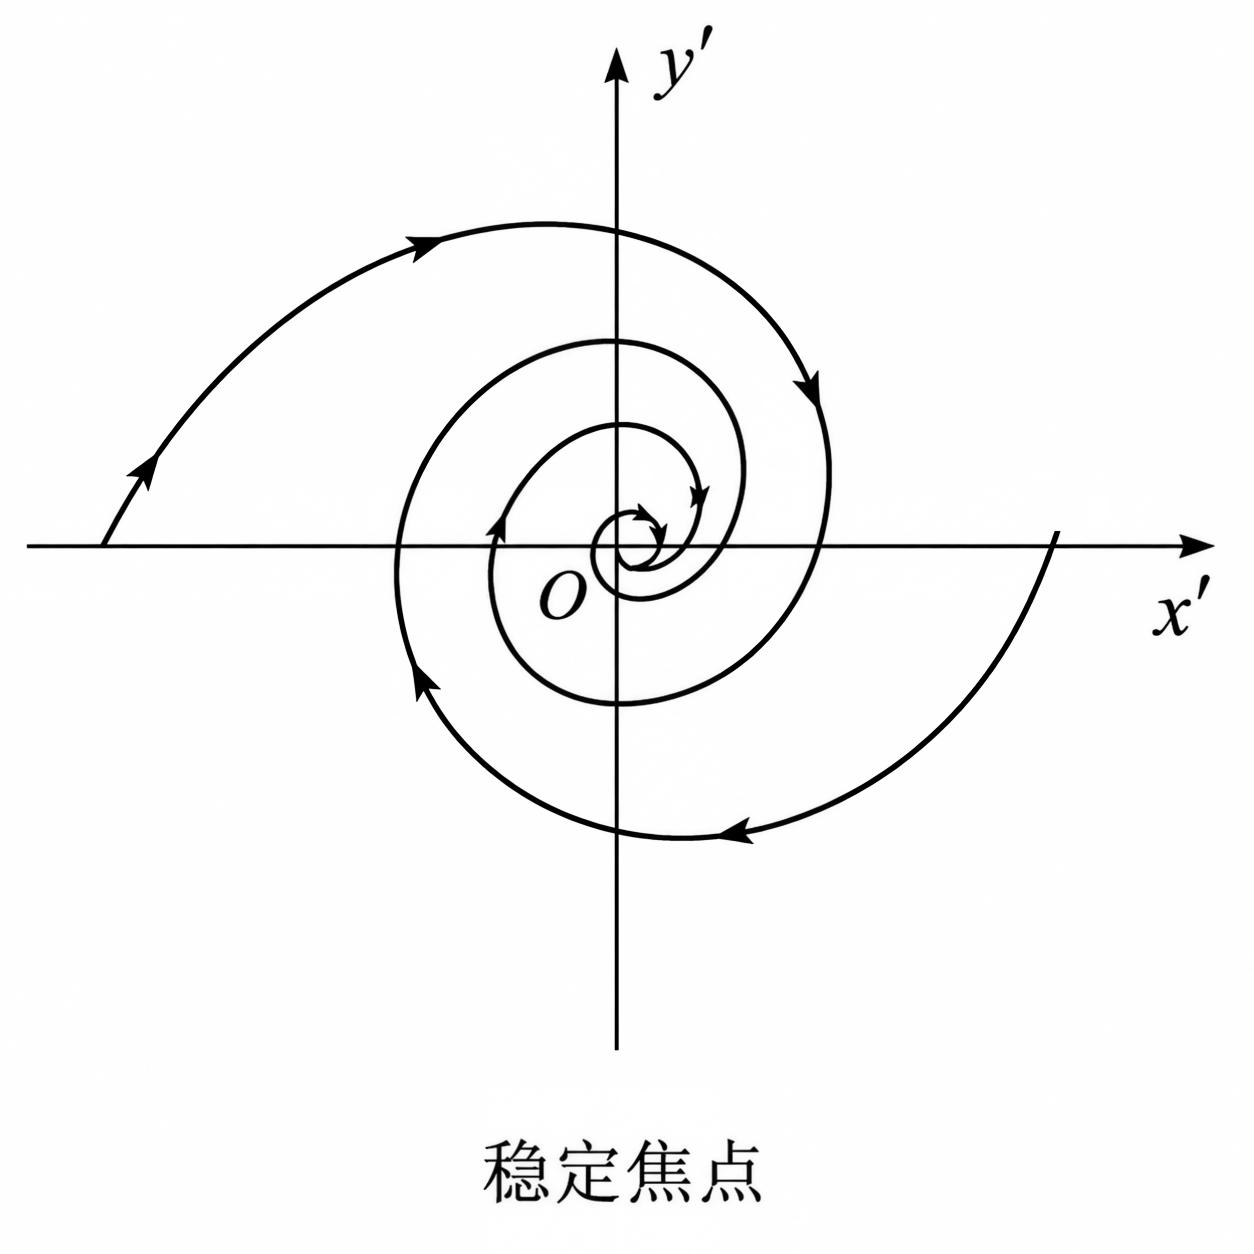
\includegraphics[width=0.4\linewidth]{figure/2.4}
	\captionof{figure}{稳定焦点}
\end{center}

\textbf{4.}\ $q>0,p<0,p^2-4q>0$。经时间反向，得到两个正实根的情形；原点为不稳定结点。

\begin{center}
	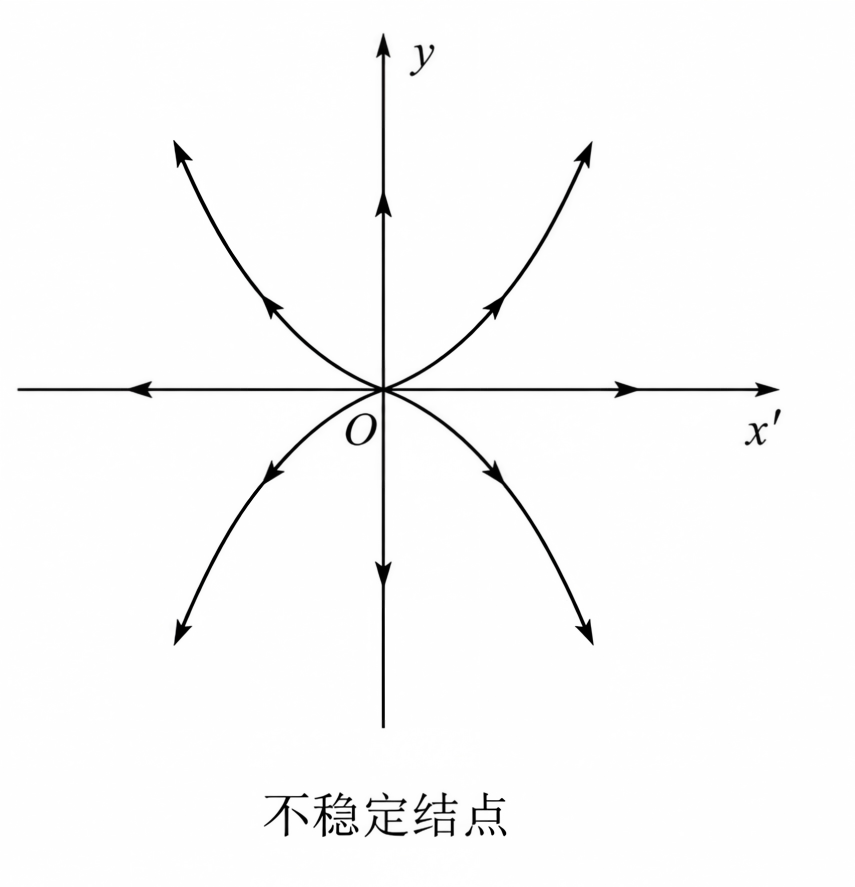
\includegraphics[width=0.4\linewidth]{figure/2.5}
	\captionof{figure}{不稳定结点}
\end{center}
\newpage

\textbf{5.}\ $q>0,p<0,p^2-4q<0$。经时间反向，原点为不稳定焦点。

\begin{center}
	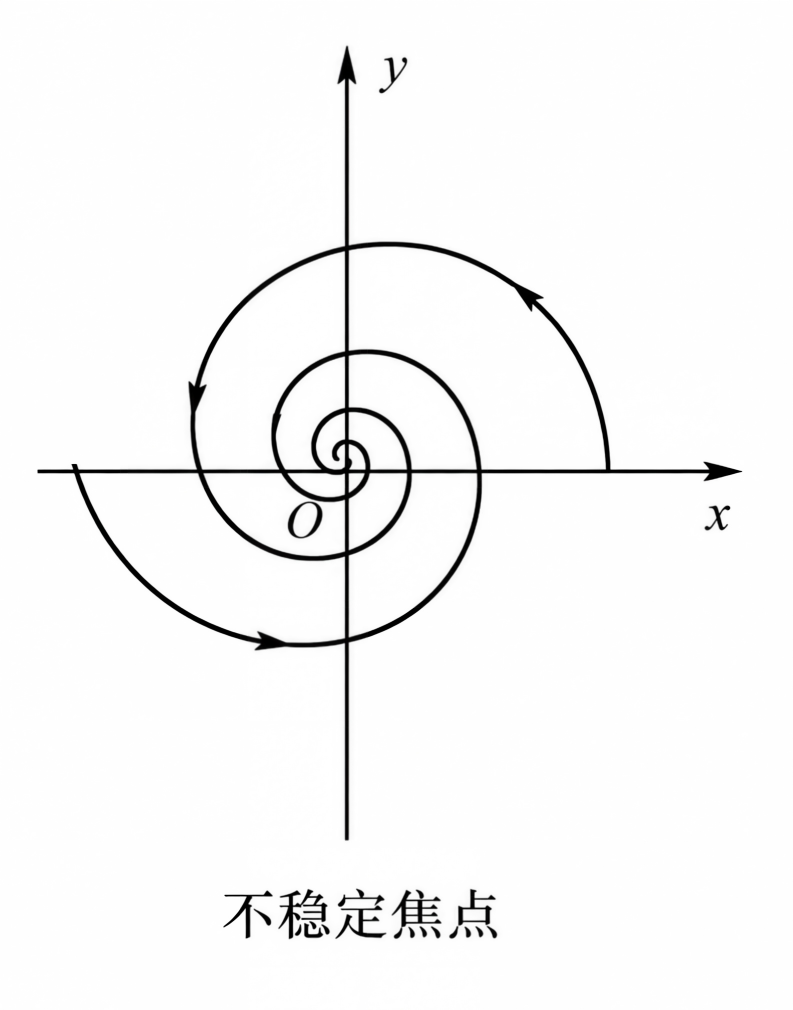
\includegraphics[width=0.4\linewidth]{figure/2.6}
	\captionof{figure}{不稳定焦点}
\end{center}

\textbf{6.}\ $q>0,p=0$。特征根为一对纯虚根；由(2.6)有 $dr/dt=0$，轨线为闭曲线，原点为中心。

\begin{center}
	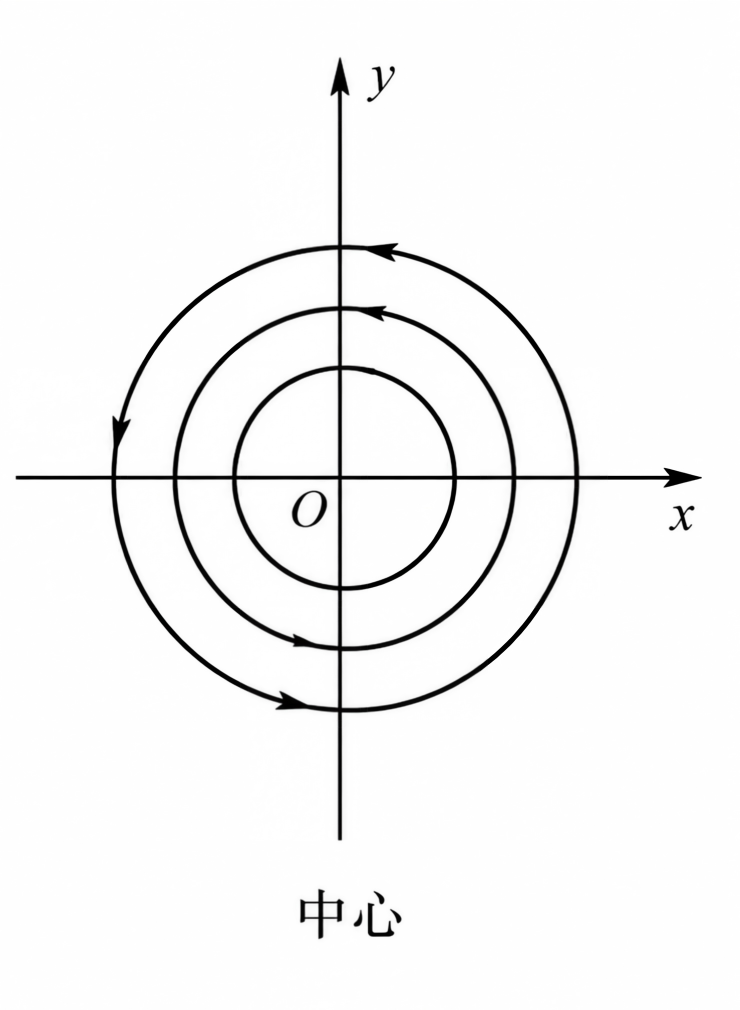
\includegraphics[width=0.4\linewidth]{figure/2.7}
	\captionof{figure}{中心}
\end{center}

\textbf{7.}\ $q>0,p>0,p^2-4q=0$。有负的重根。若最小多项式为一次式，化为 $dx'/dt=\lambda_1x'$，$dy'/dt=\lambda_1y'$，原点为稳定星形结点；若最小多项式为二次式，化为
\[
\dfrac{dx'}{dt}=\lambda_1x',\qquad
\dfrac{dy'}{dt}=\xi x'+\lambda_1y',\tag{2.8}
\]
则为稳定退化结点。
\begin{center}
	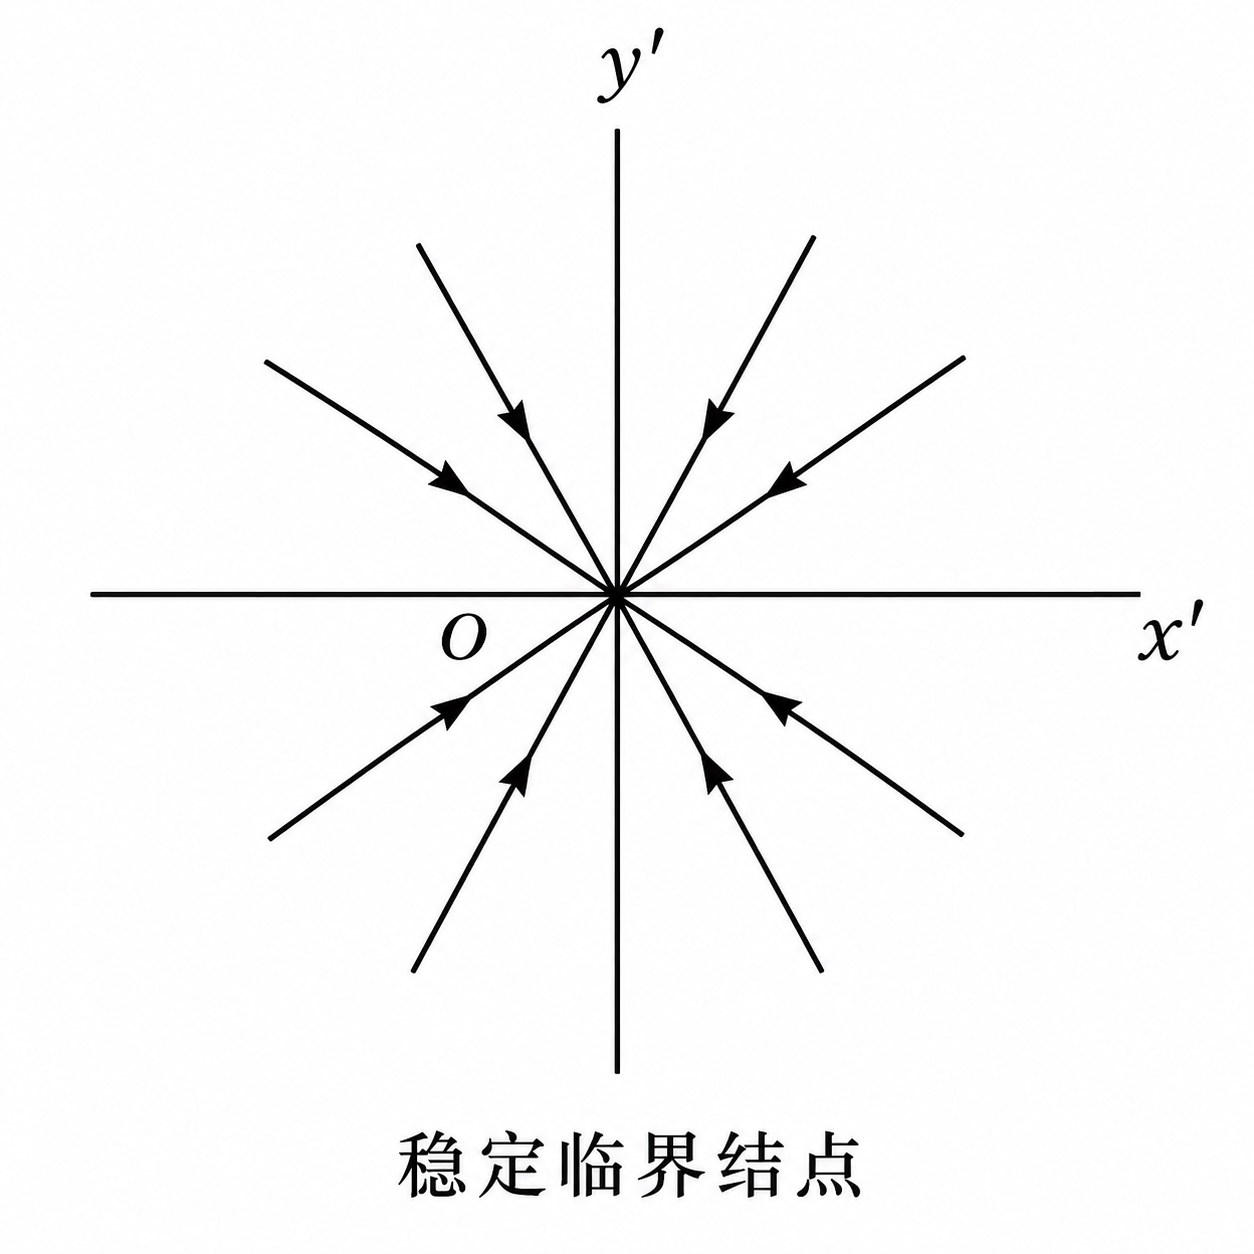
\includegraphics[width=0.4\linewidth]{figure/2.8}
	\captionof{figure}{稳定临界结点}
\end{center}



\textbf{8.}\ $q>0,p<0,p^2-4q=0$。有正的重根，轨线为第7种情形的时间反向；原点为不稳定星形结点或不稳定退化结点。
\begin{center}
	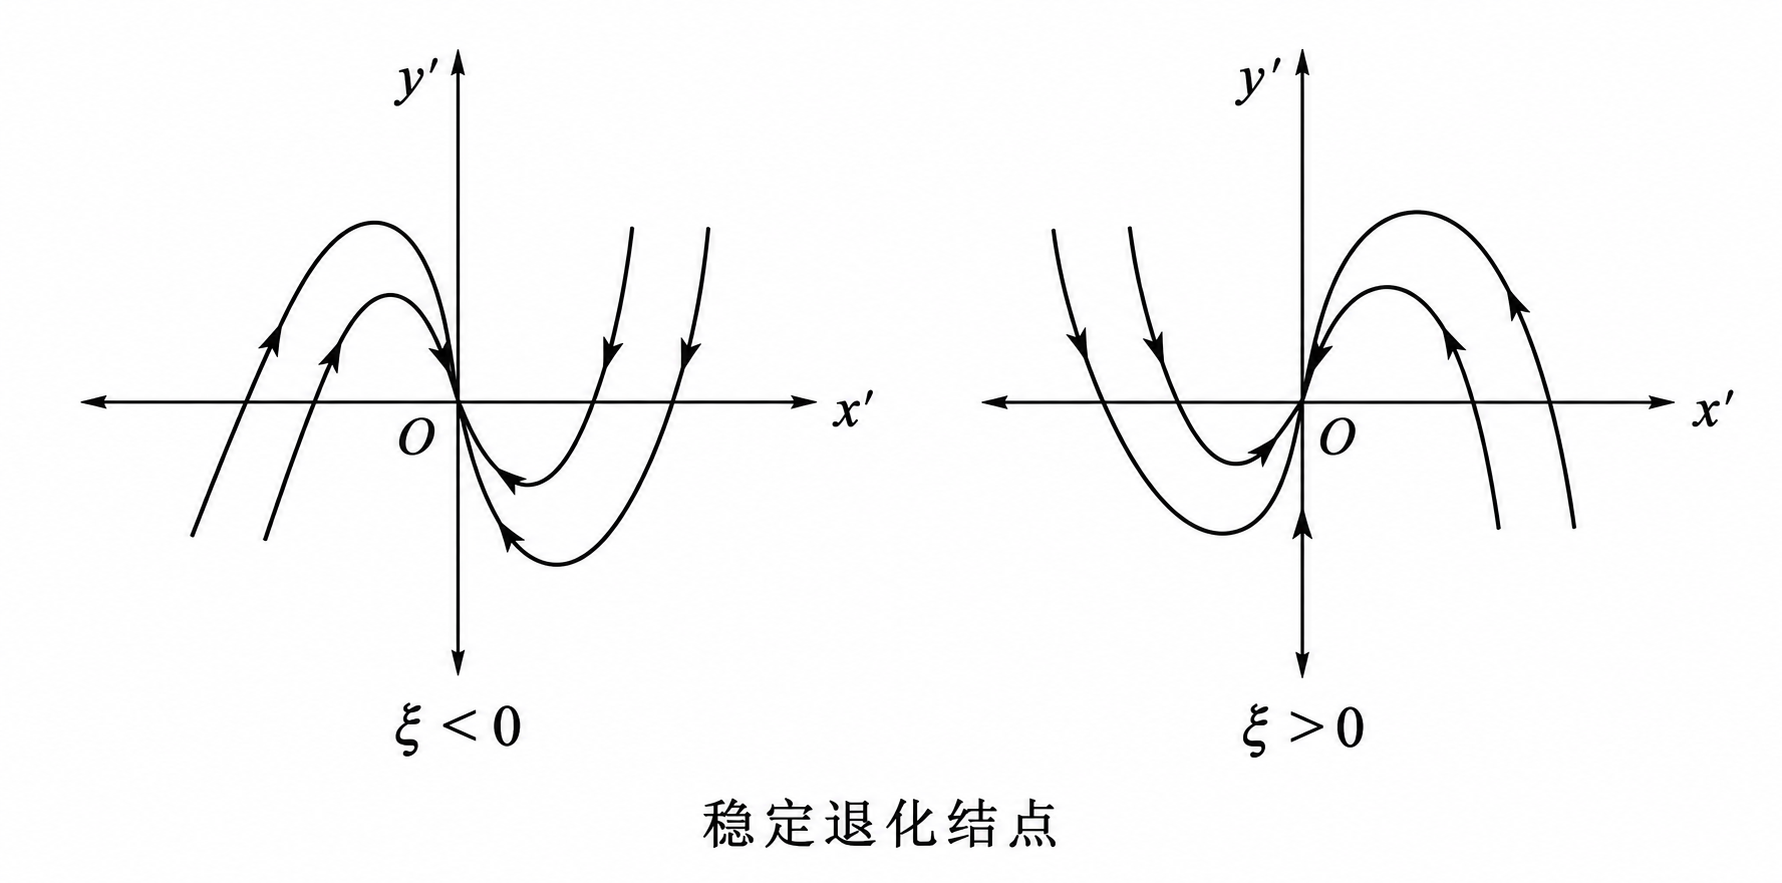
\includegraphics[width=0.47\linewidth]{figure/2.9}
	\captionof{figure}{稳定临界结点}
\end{center}
\textbf{9.}\ $q=0$。若 $a=b=c=d=0$，则平面上每一点均为奇点。若方程组中有一个方程恒为零，另一方程的零直线即为奇点的全体。若两式均不恒为零，则 $ax+by=0$ 与 $cx+dy=0$ 为同一直线，直线上的每一点均为奇点；例如在 $ac\ne0$ 时，
\[
\dfrac{dy}{dx}=\dfrac ca,\qquad ay-cx+k=0.
\]

\begin{center}
\begin{tikzpicture}[x=0.78cm,y=0.78cm,>=Stealth,font=\small]
  \begin{scope}[shift={(-3.0,0)}]
    \draw[->] (-2.0,0) -- (2.0,0) node[right] {$x$};
    \draw[->] (0,-1.45) -- (0,1.45) node[above] {$y$};
    \node[below left] at (0,0) {$O$};
    \foreach \yy in {-1.12,-.74,-.37,0,.37,.74,1.12} \fill (0,\yy) circle (1.35pt);
    \foreach \xx in {1.32,.72} \draw[->,thick] (\xx,-1.10) -- (\xx,1.10);
    \foreach \xx in {-.72,-1.32} \draw[->,thick] (\xx,1.10) -- (\xx,-1.10);
    \node[below] at (0,-1.73) {$d=0,\ c>0$};
  \end{scope}
  \begin{scope}[shift={(3.0,0)}]
    \draw[->] (-2.0,0) -- (2.0,0) node[right] {$x$};
    \draw[->] (0,-1.45) -- (0,1.45) node[above] {$y$};
    \node[below left] at (0,0) {$O$};
    \foreach \yy in {-1.12,-.74,-.37,0,.37,.74,1.12} \fill (0,\yy) circle (1.35pt);
    \foreach \xx in {-1.32,-.72} \draw[<-,thick] (\xx,-1.10) -- (\xx,1.10);
    \foreach \xx in {.72,1.32} \draw[<-,thick] (\xx,1.10) -- (\xx,-1.10);
    \node[below] at (0,-1.73) {$d=0,\ c<0$};
  \end{scope}
\end{tikzpicture}
\captionof{figure}{非孤立奇点：$d=0$}
\end{center}

\begin{center}
\begin{tikzpicture}[x=0.78cm,y=0.78cm,>=Stealth,font=\small]
  \begin{scope}[shift={(-3.0,0)}]
    \draw[->] (-2.0,0) -- (2.0,0) node[right] {$x$};
    \draw[->] (0,-1.45) -- (0,1.45) node[above] {$y$};
    \node[below left] at (0,0) {$O$};
    \draw[thick] (-1.75,0.72) -- (1.65,-0.70);
    \foreach \xx in {.70,1.28} \draw[->,thick] (\xx,-1.10) -- (\xx,1.10);
    \foreach \xx in {-1.28,-.70} \draw[->,thick] (\xx,1.10) -- (\xx,-1.10);
    \foreach \xx/\yy in {-1.28/.53,-.70/.29,0/0,.70/-.29,1.28/-.53} \fill (\xx,\yy) circle (1.35pt);
    \node[below] at (0,-1.73) {$d>0$};
  \end{scope}
  \begin{scope}[shift={(3.0,0)}]
    \draw[->] (-2.0,0) -- (2.0,0) node[right] {$x$};
    \draw[->] (0,-1.45) -- (0,1.45) node[above] {$y$};
    \node[below left] at (0,0) {$O$};
    \draw[thick] (-1.75,0.72) -- (1.65,-0.70);
    \foreach \xx in {-1.28,-.70} \draw[<-,thick] (\xx,1.10) -- (\xx,-1.10);
    \foreach \xx in {.70,1.28} \draw[<-,thick] (\xx,-1.10) -- (\xx,1.10);
    \foreach \xx/\yy in {-1.28/.53,-.70/.29,0/0,.70/-.29,1.28/-.53} \fill (\xx,\yy) circle (1.35pt);
    \node[below] at (0,-1.73) {$d<0$};
  \end{scope}
\end{tikzpicture}
\captionof{figure}{非孤立奇点：$d\ne0$}
\end{center}

上述图形是在 $(x',y')$ 平面画出的。回到 $(x,y)$ 平面，$x'=0,y'=0$ 是两条过原点的斜线，轨线的几何形状可能不同，但拓扑性质不变。将 $y=kx$ 代入(2.1)，可由
\[
bk^2+(a-d)k-c=0
\]
求得这两条直线的斜率。综合九种情形，可在 $(p,q)$ 平面画出分类图。

\begin{center}
\begin{tikzpicture}[x=1.0cm,y=0.86cm,>=Stealth,font=\scriptsize]
  \draw[->] (-3.2,0) -- (3.25,0) node[right] {$p$};
  \draw[->] (0,-1.85) -- (0,3.15) node[above] {$q$};
  \node[below left] at (0,0) {$O$};
  \draw[thick,domain=-3:3,smooth] plot (\x,{0.25*\x*\x});
  \node[anchor=west] at (2.06,2.38) {$p^2-4q=0$};
  \node[anchor=west] at (2.06,1.83) {稳定退化结点};
  \node at (1.38,0.83) {稳定焦点};
  \node at (1.67,0.22) {稳定结点};
  \node at (-1.42,0.83) {不稳定焦点};
  \node at (-1.75,0.22) {不稳定结点};
  \node[anchor=east] at (-2.25,1.66) {临界不稳定退化结点};
  \node[above] at (0,2.48) {中心};
  \node[below] at (0,-1.14) {鞍点};
  \node[below] at (1.92,0) {情形 9};
\end{tikzpicture}
\captionof{figure}{$(p,q)$ 平面上的奇点分类}
\end{center}

% ============================================================
%  §3  非线性方程组的奇点
% ============================================================
\section{非线性方程组的奇点}

给定微分方程组
\[
\left\{\begin{aligned}
\dfrac{dx}{dt}&=X(x,y),\\
\dfrac{dy}{dt}&=Y(x,y).
\end{aligned}\right.\tag{3.1}
\]
设 $O(0,0)$ 是其孤立奇点，且 $X,Y$ 在原点附近有足够高阶的连续偏导数。可写为
\[
\left\{\begin{aligned}
\dfrac{dx}{dt}&=X_m(x,y)+\Phi(x,y),\\
\dfrac{dy}{dt}&=Y_n(x,y)+\Psi(x,y),
\end{aligned}\right.\tag{3.2}
\]
其中 $X_m,Y_n$ 分别为 $x,y$ 的 $m,n$ 次齐次多项式，$m,n\ge1$，而
\[
\Phi=o(r^m),\qquad\Psi=o(r^n),\qquad r\to0.
\]
当 $m=n=1$ 且 $\Phi\equiv\Psi\equiv0$ 时，称为线性奇点；其余情形称为非线性奇点。焦点、结点、中心、鞍点称为初等奇点或简单奇点，其余的孤立奇点称为复杂奇点。

\begin{definition}{}{}
设 $L$ 是方程的轨线，点 $A(r,\theta)$ 是 $L$ 上的动点。若当 $r\to0$ 时有 $\theta\to\theta_0$，则称轨线 $L$ 沿固定方向 $\theta=\theta_0$ 进入奇点 $O$。
\end{definition}

\begin{definition}{}{}
设原点 $O$ 为方程组(3.1)的孤立奇点。若存在点列 $A_n=A(r_n,\theta_n)$，当 $n\to+\infty$ 时，$r_n\to0$，$\theta_n\to\theta_0$，且场向量的方向 $\alpha_n\to0$，则称 $\theta=\theta_0$ 为方程组(3.1)的特殊方向。
\end{definition}

若轨线沿方向 $\theta=\theta_0$ 进入奇点，则 $\theta=\theta_0$ 必为特殊方向；但沿特殊方向不一定有轨线进入奇点。对于鞍点和结点，相应的变换后方程有四个特殊方向；对于退化结点有两个特殊方向；对于临界结点，每个方向均为特殊方向；对中心和焦点没有特殊方向。

\begin{example}{}{nonlinear-special-direction}
讨论方程组
\[
\dfrac{dx}{dt}=-x,\qquad
\dfrac{dy}{dt}=-y+
\dfrac{x\cos\left|\ln\dfrac1{|x|}\right|}{\ln\dfrac1{|x|}}
\]
在奇点 $O$ 邻域内的轨线结构。
\end{example}
由第一个方程得 $x(t)=x(0)e^{-t}$。代入第二式可得
\[
y(t)=x(t)\left[C_2+\sin\left|\ln\dfrac1{|x(t)|}\right|\right].
\]
于是可适当选取 $t_n\to+\infty$，使 $dy/dx=y/x=C_2+1$。因而每一方向均为特殊方向；但除 $x=0$ 外，其余轨线均不沿固定方向进入奇点。

\chTwoFigurePlaceholder{2.13}

在极坐标下，设轨线与向量半径 $\theta=\theta_0$ 相交于点 $P$。若在点 $P$ 坐标向量与场向量的夹角 $\alpha_P<\pi$（$>\pi$），则称轨线与该半径正（负）侧相交。

\chTwoFigurePlaceholder{2.14}

由两条向量半径 $OA,OB$ 和弧 $\overset{\frown}{AB}$ 围成的扇形区域 $\overset{\frown}{OAB}$，若除 $O$ 外无其他奇点，$OA,OB$ 为无切线段，区域内至多有一个特殊方向，且边界方向不是特殊方向，则称为正常区域。轨线在两条边界上同向进入或同向离开该区域。

\chTwoFigurePlaceholder{2.15}
\chTwoFigurePlaceholder{2.16}

\begin{proposition}{}{}
若 $\overset{\frown}{OAB}$ 是第一类正常区域，则当 $t\to+\infty$ 时，由 $OA,OB$ 上每一点出发的轨线均进入奇点 $O$。
\end{proposition}

\begin{proposition}{}{}
若 $\overset{\frown}{OAB}$ 是第二类正常区域，则弧 $\overset{\frown}{AB}$ 上存在一点或一闭弧段，从其上出发的轨线当 $t\to+\infty$ 时均进入奇点 $O$。
\end{proposition}

研究非线性奇点附近轨线的定性结构，主要是找出所有特殊方向，再讨论沿这些方向是否有轨线进入奇点以及有多少条。令 $\alpha$ 为 $P(r,\theta)$ 处坐标向量与场向量的夹角，则
\[
\tan\alpha=\lim_{\Delta r\to0}r\dfrac{\Delta\theta}{\Delta r}
=r\dfrac{d\theta}{dr}.\tag{3.4}
\]
令 $x=r\cos\theta,y=r\sin\theta$，则
\[
\dfrac1r\dfrac{dr}{d\theta}=\dfrac{M(r,\theta)}{I(r,\theta)},\tag{3.5}
\]
其中，若 $m>n$、$m<n$、$m=n$，分别令
\[
G(\theta)=\cos\theta Y_n(\cos\theta,\sin\theta),\quad
G(\theta)=-\sin\theta X_m(\cos\theta,\sin\theta),
\]
或
\[
G(\theta)=\cos\theta Y_n(\cos\theta,\sin\theta)-\sin\theta X_m(\cos\theta,\sin\theta).\tag{3.6}
\]
由附加项的条件，在充分小的 $r$ 下，上式右端的分母除以相应的 $r^m$ 或 $r^n$ 后为 $G(\theta)+o(1)$。故特殊方向必须是示性方程 $G(\theta)=0$ 的根。

\begin{theorem}{}{}
若原点为方程组(3.1)的孤立奇点，且 $X,Y$ 在原点邻域内解析，则若有轨线进入原点，它只能螺旋形地进入或沿固定方向进入。
\end{theorem}

\section{特征根实部不为0时附加非线性项的情形}

本节研究在线性方程组的右端附加非线性项后，当特征根实部不为零时奇点附近轨线的拓扑结构和定性结构是否保持不变。给定线性方程组
\[
\left\{\begin{aligned}
\dfrac{dx}{dt}&=ax+by,\\
\dfrac{dy}{dt}&=cx+dy,
\end{aligned}\right.\tag{4.1}
\]
及方程组
\[
\left\{\begin{aligned}
\dfrac{dx}{dt}&=ax+by+\Phi(x,y),\\
\dfrac{dy}{dt}&=cx+dy+\Psi(x,y),
\end{aligned}\right.\tag{4.2}
\]
其中 $a,b,c,d$ 为实数，$\Phi(0,0)=\Psi(0,0)=0$，并引入条件：
\[
\Phi(x,y),\Psi(x,y)=o(r),\qquad r\to0,\tag{4.3}
\]
以及 $\Phi,\Psi$ 在原点小邻域内对 $x,y$ 连续可微。第二个条件还保证了解的存在唯一性。

\begin{definition}{}{}
若存在 $\delta>0$，使任一满足 $x^2(t_0)+y^2(t_0)<\delta$ 的解在 $t\to+\infty$ 时满足 $x^2(t)+y^2(t)\to0$，则称 $O(0,0)$ 为稳定吸引子；时间反向时称为不稳定吸引子。
\end{definition}

\begin{theorem}{}{}
若 $O(0,0)$ 是方程组(4.1)的稳定（不稳定）吸引子，且方程组(4.2)的附加项满足(4.3)，则 $O(0,0)$ 也是方程组(4.2)的稳定（不稳定）吸引子。
\end{theorem}

证明中可取
\[
V(x,y)=(ad-bc)(x^2+y^2)+(ay-cx)^2+(by-dx)^2.
\]
当 $ad-bc>0$ 且 $-(a+d)>0$（或小于零）时，$V(0,0)=0$，在原点外 $V(x,y)>0$，并且沿(4.1)、(4.2)的导数分别具有相应符号，故结论成立。

\begin{theorem}{}{}
若 $O(0,0)$ 是方程组(4.1)的稳定（不稳定）焦点，且条件(4.3)成立，则 $O(0,0)$ 也是方程组(4.2)的稳定（不稳定）焦点。
\end{theorem}

经非退化线性变换，若线性部分有共轭复特征根，可化为
\[
\left\{\begin{aligned}
\dfrac{dx'}{dt}&=\mu_1x'+\mu_2y'+\Phi'(x',y'),\\
\dfrac{dy'}{dt}&=-\mu_2x'+\mu_1y'+\Psi'(x',y').
\end{aligned}\right.\tag{4.4}
\]
其示性方程无实根，故原点只能为中心或焦点；再由前一结论，原点为同稳定性的焦点。

若线性部分有两个非零实特征根，经非退化线性变换可化为
\[
\left\{\begin{aligned}
\dfrac{dx'}{dt}&=\lambda_1x'+\Phi'(x',y'),\\
\dfrac{dy'}{dt}&=\lambda_2y'+\Psi'(x',y').
\end{aligned}\right.\tag{4.5}
\]
其中 $\Phi',\Psi'$ 仍满足相应的条件。

\begin{theorem}{}{}
设 $O(0,0)$ 是方程组(4.1)的正常结点，$|\lambda_2|>|\lambda_1|$。

\noindent (i) 若条件(4.3)成立，则方程组(4.5)在奇点附近的轨线都沿特殊方向 $\theta=0,\pi/2,\pi,3\pi/2$ 进入奇点；

\noindent (ii) 若附加项连续可微，则沿 $\theta=\pi/2,3\pi/2$ 各只有一条轨线进入奇点。
\end{theorem}

\begin{theorem}{}{}
设 $O(0,0)$ 是方程组(4.1)的鞍点，$\lambda_1>0>\lambda_2$。

\noindent (i) 若条件(4.3)成立，则方程组(4.5)有轨线当 $t\to+\infty$ 时沿 $\theta=\pi/2,3\pi/2$ 进入奇点；有轨线当 $t\to-\infty$ 时沿 $\theta=0,\pi$ 进入奇点，其余轨线双侧离开充分小的邻域；

\noindent (ii) 若附加项连续可微，则沿四个特殊方向各只有一条轨线进入奇点。
\end{theorem}

\begin{theorem}{}{}
设 $O(0,0)$ 是方程组(4.1)的临界结点。若方程组(4.2)中的附加项满足
\[
\Phi(x,y),\Psi(x,y)=o\bigl(r^{1+\varepsilon}\bigr),\qquad r\to0,
\]
其中 $\varepsilon>0$ 为任意小的正数，则方程组(4.2)沿任意方向 $\theta=\theta_0$ 有唯一的轨线进入奇点 $O$。
\end{theorem}

\begin{theorem}{}{}
设 $O(0,0)$ 是方程组(4.1)的退化结点。若方程组(4.2)的附加项满足上述条件，则 $O(0,0)$ 也是方程组(4.2)的退化结点。
\end{theorem}

\begin{example}{}{critical-node-counterexample}
讨论方程组
\[
\left\{\begin{aligned}
\dfrac{dx}{dt}&=-x-\dfrac{2y}{\ln(x^2+y^2)},\\
\dfrac{dy}{dt}&=-y-\dfrac{2x}{\ln(x^2+y^2)}.
\end{aligned}\right.\tag{4.6}
\]
的原点附近轨线结构。
\end{example}
令 $x=r\cos\theta,y=r\sin\theta$，则
\[
\dfrac{d\theta}{dt}=-\dfrac1{\ln r},\qquad
\dfrac{dr}{dt}=-r.\tag{4.7}
\]
于是 $r(t)=r(0)e^{-t}$，且
\[
\theta(t)-\theta(0)=\ln\ln\dfrac1{r(t)}-\ln\ln\dfrac1{r(0)}.
\]
故 $r(t)\to0$、$\theta(t)\to+\infty$；原点为焦点，而相应的线性方程的原点为临界结点。该例的附加项满足条件1、2，但不满足上述较强条件。

\begin{example}{}{degenerate-node-counterexample}
讨论方程组
\[
\left\{\begin{aligned}
\dfrac{dx}{dt}&=-x,\\
\dfrac{dy}{dt}&=-y+\dfrac{x}{\ln\dfrac1{|x|}}.
\end{aligned}\right.\tag{4.8}
\]
由 $x(t)=x(0)e^{-t}$ 得
\[
y(t)=x(t)\left[C_2+\ln\ln\dfrac1{|x(t)|}\right].
\]
所以 $x(t),y(t)\to0$，但 $y(t)/x(t)\to+\infty$。因此原点为稳定吸引子，且轨线均沿 $y$ 轴进入原点，即为退化结点；相应线性方程的原点则为临界结点。
\end{example}

% ============================================================
%  §5  特征根是一对纯虚根时附加非线性项的情形(中心和焦点判别)
% ============================================================
\section{特征根是一对纯虚根时附加非线性项的情形(中心和焦点判别)}
设线性部分的特征根为 $\pm\mu i$，$\mu>0$。经线性变换后，线性方程组及附加非线性项的方程组分别为
\[
\dfrac{dx'}{dt}=\mu y',\qquad \dfrac{dy'}{dt}=-\mu x',
\tag{5.1}
\]
\[
\dfrac{dx'}{dt}=\mu y'+\Phi'(x',y'),\qquad
\dfrac{dy'}{dt}=-\mu x'+\Psi'(x',y').
\tag{5.2}
\]
其中 $\Phi',\Psi'$ 仍满足本章第4节的附加项条件。

\begin{theorem}{}{pure-imaginary}
在上述条件下，原点 $O$ 或为中心，或为焦点，或为中心焦点。
\end{theorem}

\begin{example}{}{focus-example}
讨论方程组
\[
\dfrac{dx}{dt}=-y-x(x^2+y^2),\qquad
\dfrac{dy}{dt}=x-y(x^2+y^2).
\tag{5.3}
\]
令 $x=r\cos\theta,\ y=r\sin\theta$，得
\[
\dfrac{d\theta}{dt}=1,\qquad \dfrac{dr}{dt}=-r^3.
\]
故
\[
\theta=\theta_0+t,\qquad
r=\left(2t+\dfrac1{r^2(0)}\right)^{-\frac12}.
\]
原点为稳定焦点。
\end{example}

\begin{example}{}{centre-focus-example}
讨论方程组
\[
\begin{aligned}
\dfrac{dx}{dt}&=-y+x(x^2+y^2)^k
 \sin\dfrac{\pi}{\sqrt{x^2+y^2}},\\
\dfrac{dy}{dt}&=x+y(x^2+y^2)^k
 \sin\dfrac{\pi}{\sqrt{x^2+y^2}}.
\end{aligned}
\tag{5.4}
\]
极坐标方程为
\[
\dfrac{d\theta}{dt}=1,\qquad
\dfrac{dr}{dt}=r^{2k+1}\sin\dfrac{\pi}{r}.
\]
圆周 $r=1/n\ (n=1,2,\ldots)$ 都是闭轨线；相邻圆周之间又有非闭轨线。因此原点为中心焦点。
\end{example}

\subsection*{中心和焦点的判别法一}

\begin{lemma}{}{periodic-integral}
若连续函数 $h(x)$ 以 $l$ 为周期，则
\[
\int_0^x h(\xi)\,d\xi=gx+\varphi(x),\qquad
g=\dfrac1l\int_0^l h(\xi)\,d\xi,
\]
其中 $\varphi(x+l)=\varphi(x)$。
\end{lemma}

在极坐标中，方程组可写为
\[
\dfrac{d\theta}{dt}=-\mu+Q(r,\theta),\qquad
\dfrac{dr}{dt}=rR(r,\theta),
\tag{5.5}
\]
从而
\[
\dfrac{dr}{d\theta}
 =R_2(\theta)r^2+R_3(\theta)r^3+\cdots .
\tag{5.6}
\]
这里 $R_i(\theta)$ 都以 $2\pi$ 为周期。取初值 $r(0,c)=c$，其解析解为
\[
r(\theta,c)=r_1(\theta)c+r_2(\theta)c^2+\cdots ,
\tag{5.8}
\]
其中
\[
r_1=1,\qquad r_2=\int_0^\theta R_2(s)\,ds,\qquad
r_3=\int_0^\theta\bigl[R_3(s)+2R_2(s)r_2(s)\bigr]\,ds .
\]
依引理可写成 $r_i=g_i\theta+\varphi_i(\theta)$。若所有 $g_i=0$，则原点为中心；若 $g_m$ 是第一个非零数，则原点为焦点，且其稳定性由 $g_m$ 的符号决定。

\subsection*{中心和焦点的判别法二}

设
\[
\dfrac{dx}{dt}=y+\sum_{k=2}^{\infty}\Phi_k,\qquad
\dfrac{dy}{dt}=-x+\sum_{k=2}^{\infty}\Psi_k.
\tag{5.16}
\]
寻求形式幂级数
\[
F=x^2+y^2+\sum_{k=3}^{\infty}F_k
\]
使得沿轨线 $dF/dt=0$。比较齐次项可得递推关系
\[
\begin{aligned}
xF_{n,y}-yF_{n,x}
={}&2(x\Phi_{n-1}+y\Psi_{n-1})\\
&+\sum_{k=3}^{n-1}
 \bigl(\Phi_{n-k+1}F_{k,x}+\Psi_{n-k+1}F_{k,y}\bigr).
\end{aligned}
\tag{5.18}
\]
若各级方程均可解，则原点为中心；否则，设第一次出现不相容条件时得到
\[
\dfrac{d}{dt}(x^2+y^2+F_3+\cdots+F_{2m})
 =-\lambda r^{2m}+O(r^{2m+1}),
\tag{5.26}
\]
则 $\lambda>0$ 时原点为稳定焦点，$\lambda<0$ 时为不稳定焦点。

若方程组关于一条坐标轴具有镜像对称性，例如
\[
Y(-x,y)=Y(x,y),\qquad X(-x,y)=-X(x,y),
\]
则原点为中心。

对于二次系统
\[
\begin{aligned}
\dfrac{dx}{dt}&=-y+a_{20}x^2+a_{11}xy+a_{02}y^2,\\
\dfrac{dy}{dt}&=x+b_{20}x^2+b_{11}xy+b_{02}y^2,
\end{aligned}
\tag{5.28}
\]
令
\[
\begin{gathered}
A=a_{20}+a_{02},\quad B=b_{20}+b_{02},\\
\alpha=a_{11}+2b_{02},\quad \beta=b_{11}+2a_{20},\\
\gamma=b_{20}A^3-(a_{20}-b_{11})A^2B
 +(b_{02}-a_{11})AB^2-a_{02}B^3,\\
\delta=a_{02}^2+b_{20}^2+a_{02}A+b_{20}B.
\end{gathered}
\tag{5.30}
\]
则相应的焦点量为
\[
\begin{aligned}
W_1&=A\alpha-B\beta,\\
W_2&=[\beta(5A-\beta)+\alpha(5B-\alpha)]\gamma,\\
W_3&=(A\beta+B\alpha)\gamma\delta.
\end{aligned}
\tag{5.29}
\]
原点为 $k$ 阶细焦点 $(k=1,2,3)$，当且仅当此前的焦点量为零而 $W_k\ne0$；$W_k<0$ 时稳定，$W_k>0$ 时不稳定。原点为中心当且仅当下列三组条件之一成立：
\[
\begin{array}{ll}
(1)&A\alpha-B\beta=\gamma=0;\\
(2)&\alpha=\beta=0;\\
(3)&5A-\beta=5B-\alpha=\delta=0.
\end{array}
\]

% ============================================================
%  §6  奇点的几何分类
% ============================================================
\section{奇点的几何分类}
本节讨论非中心孤立奇点邻域内轨线的几何形状。

\begin{theorem}{}{no-closed-orbit}
设 $O$ 为非中心孤立奇点，则存在充分小的圆盘 $S_\delta$，使其中除 $O$ 外没有奇点，也没有包围 $O$ 的整条闭轨线。
\end{theorem}

\chTwoFigurePlaceholder{2.28}

\begin{theorem}{}{semi-orbits}
在奇点 $O$ 的任一充分小邻域中，至少有两条半轨线在 $t\to+\infty$ 或 $t\to-\infty$ 时趋于 $O$。
\end{theorem}

\begin{theorem}{}{local-orbits}
可取充分小的 $S_\delta$，使其中每一条正、负半轨线或者趋于 $O$，或者离开 $S_\delta$。
\end{theorem}

\chTwoFigurePlaceholder{2.29}

一条经过邻域内点的轨线按两端的性状分为三种：一端进入而另一端离开 $O$ 的称为双曲型；两端均离开 $O$ 的称为双曲扇形型；两端均进入 $O$ 的称为椭圆型。由两条趋于 $O$ 的半轨线及其间的弧段所围成的区域称为曲边扇形。

\chTwoFigurePlaceholder{2.30}

\begin{theorem}{}{sector-finiteness}
在充分小的邻域内，双曲扇形、双曲椭圆扇形及椭圆扇形的数目均为有限。
\end{theorem}

因此，孤立奇点邻域内的曲边扇形只有五种：椭圆扇形、双曲扇形、双曲椭圆扇形、双曲型扇形和双曲椭圆型扇形。

\chTwoFigurePlaceholder{2.31}

设 $e$ 为椭圆扇形数，$h$ 为双曲扇形和双曲椭圆扇形的总数，奇点的指数为 $I$，则 Bendixson 公式为
\[
I=1+\dfrac{e-h}{2}.
\]

\begin{definition}{}{separatrix}
若趋于奇点的半轨线的任何充分小邻域内都含有不趋于该奇点的轨线，则称此半轨线为分界线。
\end{definition}

\begin{example}{}{geometric-classification}
讨论方程组
\[
\dfrac{dx}{dt}=-x^2+2xy,\qquad
\dfrac{dy}{dt}=\dfrac32y^2-\dfrac12x^2
\]
在原点邻域内的轨线结构。
\end{example}

% ============================================================
%  §7  有零特征根时附加非线性项的情形
% ============================================================
\section{有零特征根时附加非线性项的情形}
+本节设线性部分至少有一个零特征根，且线性项不全为零。

先设一个特征根为零，另一个不为零。经线性变换后可写为
\[
\dfrac{dx}{dt}=P_2(x,y),\qquad
\dfrac{dy}{dt}=y+Q_2(x,y),
\tag{7.1}
\]
其中 $P_2,Q_2$ 的展开式从二次项开始。由
\[
y+Q_2(x,y)=0
\]
可解得 $y=\varphi(x)$，且 $\varphi(0)=\varphi'(0)=0$。设
\[
\varphi(x)=a_mx^m+\cdots,\qquad a_m\ne0.
\]

\begin{theorem}{}{one-zero-eigenvalue}
对于方程组(7.1)，有：

\noindent (i) 当 $m$ 为奇数、$a_m>0$ 时，原点为不稳定结点；

\noindent (ii) 当 $m$ 为奇数、$a_m<0$ 时，原点为鞍点，具有四条分界线；

\noindent (iii) 当 $m$ 为偶数时，原点为鞍结点；它有两条切于非零特征方向的分界线和一个抛物扇形，另有两个双曲扇形。
\end{theorem}

\chTwoFigurePlaceholder{2.32}
\chTwoFigurePlaceholder{2.33}
\chTwoFigurePlaceholder{2.34}
\chTwoFigurePlaceholder{2.35}

现设两个特征根均为零，但线性部分不为零。经过可逆变换，方程组可化为
\[
\dfrac{dx}{dt}=y,\qquad \dfrac{dy}{dt}=\overline Q_2(x,y).
\tag{7.6}
\]
其右端可写为
\[
\dfrac{dx}{dt}=y,\qquad
\dfrac{dy}{dt}=a_kx^k[1+h(x)]
+b_nx^ny[1+g(x)]+y^2p(x,y),
\tag{7.7}
\]
其中 $h(0)=g(0)=0$，$a_k\ne0$。

令 $k=2m+1$。若 $b_n=0$ 或 $n>m$，则
\[
a_{2m+1}<0\ \Longrightarrow\ \text{中心或焦点},\qquad
a_{2m+1}>0\ \Longrightarrow\ \text{鞍点}.
\]
当 $b_n\ne0,\ n<m$ 时，$a_{2m+1}>0$ 仍为鞍点；当 $a_{2m+1}<0$ 时，$n$ 为偶数对应结点，$n$ 为奇数对应一个椭圆扇形和一个双曲扇形。

\chTwoFigurePlaceholder{2.36}
\chTwoFigurePlaceholder{2.37}
\chTwoFigurePlaceholder{2.38}
\chTwoFigurePlaceholder{2.39}
\chTwoFigurePlaceholder{2.40}
\chTwoFigurePlaceholder{2.41}
\chTwoFigurePlaceholder{2.42}
\chTwoFigurePlaceholder{2.43}
\chTwoFigurePlaceholder{2.44}
\chTwoFigurePlaceholder{2.45}

若 $n=m$，令
\[
\lambda=b_n^2+4(m+1)a_{2m+1}.
\]
上述分类中相应条件改为由 $\lambda$ 的符号判定。综上可得：当 $a_{2m+1}>0$ 时为鞍点；当 $a_{2m+1}<0$ 且 $b_n=0$，或 $n>m$，或 $n=m,\lambda<0$ 时为中心或焦点；当 $a_{2m+1}<0$ 且 $n\le m,\lambda\ge0$ 时，按 $n$ 的奇偶分别为结点或由一个椭圆扇形和一个双曲扇形组成的奇点。

\chTwoFigurePlaceholder{2.46}
\chTwoFigurePlaceholder{2.47}
\chTwoFigurePlaceholder{2.48}
\chTwoFigurePlaceholder{2.49}

\begin{theorem}{}{even-k}
当 $k=2m$ 时，若 $b_n=0$，则原点为退化奇点；若 $b_n\ne0$ 且 $n\ge m$，则原点为鞍结点。
\end{theorem}

\chTwoFigurePlaceholder{2.50}
\chTwoFigurePlaceholder{2.51}

实际计算时，先由 $y+P_2(x,y)=0$ 求出 $y=\varphi(x)$，再计算
\[
\psi(x)=Q_2(x,\varphi(x)),\qquad
\delta(x)=P_{2x}(x,\varphi(x))+Q_{2y}(x,\varphi(x)).
\]
由 $\psi,\delta$ 展开式中的最低次非零项，即可确定上述判别中的 $k,m,a_k,n,b_n$。

\begin{example}{}{zero-eigenvalue-example1}
讨论方程组
\[
\dfrac{dx}{dt}=x(-y+y^2+3xy),\qquad
\dfrac{dy}{dt}=3x+y-x^2+y^3+3xy^2.
\]
原点可化为(7.1)的类型，并由定理 \ref{thm:one-zero-eigenvalue} 判定其局部轨线结构。
\end{example}

\begin{example}{}{zero-eigenvalue-example2}
讨论方程组
\[
\dfrac{dx}{dt}=y-\dfrac12xy-3x^3,\qquad
\dfrac{dy}{dt}=-y\left(x+\dfrac32y\right).
\]
它在原点邻域内的图形为图2.52所示的类型。
\end{example}

\chTwoFigurePlaceholder{2.52}

\begin{example}{}{zero-eigenvalue-example3}
讨论方程组
\[
\dfrac{dx}{dt}=y+y^2-x^3,\qquad
\dfrac{dy}{dt}=3x^2y+y^3-3x^5.
\]
其原点邻域的轨线结构如图2.53所示。
\end{example}

\chTwoFigurePlaceholder{2.53}
\chTwoFigurePlaceholder{2.54}

% ============================================================
%  习题和参考文献
% ============================================================
\section*{习题和参考文献}
\subsection*{习题}

\begin{enumerate}
\item 试画出第2节情形9(iii)的草图。
\item 试讨论下列非线性方程组在奇点 $O(0,0)$ 邻域轨线的结构，并画出草图：
\[
\begin{array}{ll}
\text{(i)}&
\dfrac{dx}{dt}=-x+e^{-y}-1,\qquad
\dfrac{dy}{dt}=1-e^{x+y};\\[4pt]
\text{(ii)}&
\dfrac{dx}{dt}=xy,\qquad
\dfrac{dy}{dt}=y^2+x^4;\\[4pt]
\text{(iii)}&
\dfrac{dx}{dt}=-x^6,\qquad
\dfrac{dy}{dt}=y^3-x^4y.
\end{array}
\]
\item 试证例题3.1，4.1，4.2，4.3中的附加项满足条件1和条件2，但不满足条件 $1^\ast$。
\item 试证定理4.5仍真，若将条件 $1^\ast$ 换成条件 $1^{\ast\ast}$：
\[
|\Phi(x,y)|,\ |\Psi(x,y)|<\eta(r),\qquad r\le r_1,
\]
其中 $\eta(r)\in C^0(0\le r\le r_1)$，$\eta(r)=o(r)$ $(r\to0)$，且
\[
\int_0^{r_1}\dfrac{\eta(r)}{r^2}\,dr<+\infty.
\]
\item 试讨论，若将条件 $1^\ast$ 换成条件 $1^{\ast\ast}$，定理4.6是否仍真。
\item 试用第一判别法和第二判别法来判定方程组
\[
\dfrac{dx}{dt}=-y+xy+2y^2,\qquad
\dfrac{dy}{dt}=x+3x^2+y^3
\]
的奇点 $O(0,0)$ 是中心或焦点。
\item 试证若 $O(0,0)$ 是方程组(5.16)的焦点，则第一判别法中使 $g_n\ne0$ 的最小正整数 $n$ 与第二判别法中使(5.19)无解的最小偶数 $2m$ 之间有关系 $2m=n+1$。
\item 试讨论下列非线性方程组在奇点 $O(0,0)$ 邻域轨线的结构，并画出草图：
\[
\begin{array}{ll}
\text{(i)}&
\dfrac{dx}{dt}=-4x^2+2xy,\qquad
\dfrac{dy}{dt}=y^3-2x^3+x^4;\\[4pt]
\text{(ii)}&
\dfrac{dx}{dt}=2x^3+x^2y+x^2,\qquad
\dfrac{dy}{dt}=2xy^2-x^3+2y^2.
\end{array}
\]
\item 试讨论下列非线性方程组在奇点 $O(0,0)$ 邻域轨线的结构，并画出草图：
\[
\dfrac{dx}{dt}=x(2y+x),\qquad
\dfrac{dy}{dt}=x+2xy+y^2.
\]
\end{enumerate}

\subsection*{参考文献}

\begin{enumerate}
\item Вайсборд, С.\ М., Об эквивалентности систем дифференциальных уравнений в окрестности особой точки, \textit{Научные Доклады Высшей Школы, Физ-Матем. Науки}, 1958, 1, 37--42.
\item Lohn, R., Über singuläre Punkte gewöhnlicher Differentialgleichungen, \textit{Math. Ztscher.}, 44(1939), 4, 507--535.
\item 张锦炎，常微分方程几何理论和分支问题，北京大学出版社，1981。
\item 胡钦训，陆毓勋，高次奇点在不定号情形下的定性分析，\textit{北京工业学院学报}，1981，2，1--16。
\item Гробман, Д., О гомеоморфизме систем дифференциальных уравнений, \textit{ДАН СССР}, 128(1959), 880--881.
\item Hartman, P., On the local linearization of differential equations, \textit{Proc. A. M. S.}, 14(1963), 568--573.
\item Sternberg, S., Lectures on differential geometry, Prentice-Hall, 1964.
\item Ляпунов, А.\ М., Исследование одного из особенных случаев задачи об устойчивости движения, \textit{Мат. Сб.}, 17(1893), 2.
\item Альмухамедов, М.\ И., О числе возможных типов особых точек для систем обыкновенных дифференциальных уравнений с $n$-переменными, \textit{Казань, Изв. Физматем. общества}(3), 8(1936--1937), 23--29.
\item ---，О проблеме центра，---，8(1936--1937)，29--37。
\item 廖山涛，常微系统的结构稳定性及一些相关的问题，\textit{计算机应用与应用数学}，7(1978)，52--64。
\item Dulac, H., Détermination et intégration d'une certaine classe d'équations différentielles ayant pour point singulier un centre, \textit{Bull. Sc. Math.} (2), 32(1908), 230--252.
\item Kapteyn, W., Over de middelpunten de integraalkrommen van differentiaalvergelijkingen van de eerste orde en den eersten graad, \textit{Koninkl. Nederland. Akad.}, 19(1911), 1446--1457.
\item ---，Nieuw onderzoek omtrent de middelpunten der integralen van differentiaalvergelijkingen van de eerste orde en den eersten graad，\textit{Koninkl. Nederland. Akad.}, 20(1912), 1354--1365; 21(1912), 27--33.
\item Сахарников, Н.\ А., Об условиях фроммера существования центра, \textit{ПММ}, 12:5(1948), 669--670.
\item Сибирский, К.\ С., Алгебраические инварианты дифференциальных уравнений и матриц, Кишинев, Штиинца, 1976, 131--140.
\item Баутин, Н.\ Н., О числе предельных циклов, появляющихся при изменении коэффициентов из состояния равновесия типа фокуса или центра, \textit{Мат. Сб.}, 30(72), 1952, 1, 181--196.
\item 葉元勋，刘海全，微分方程公式的机器推导(III)，\textit{科学通报}，7(1981)，388--391。
\item 李承治，关于平面二次系统的两个问题，\textit{中国科学，A辑}，12(1982)，1087--1096。
\item 叶澄谦，В.\ И.\ Зубов著“A.\ М.\ Ляпунов方法及其应用”一书中两个错误定理的修正，\textit{南京大学学报}，1(1963)，67--70。
\item 黄文灿，Cauchy 运动和极小集合，\textit{数学学报}，22(1979)，249--252。
\item 丁同仁，关于 Ляпунов 第一临界情形积分曲线的拓扑分布，见第一章文献[3]，138--146。
\item Андронов, А.\ А., Леонтович, Е.\ А., Гордон, И.\ И., Майер, А.\ Г., Качественная теория динамических систем второго порядка, Изд. Наука, 1966, 241--249, 377--410.
\item Frömmer, M., Die Integralkurven einer gewöhnlichen Differentialgleichung erster Ordnung in der Umgebung rationaler Unbestimmtheitsstellen, \textit{Math. Annulen}, 99(1928), 222--272.
\item Андреев, А.\ Ф., Особые точки дифференциальных уравнений, Минск, Высшая школа, 1979.
\end{enumerate}

\endinput
